%***********************************************************************************
%*       OOA
%***********************************************************************************
\part{OOA - Objektorientierte Analyse}
\newpage
\section{Gui-Prototyp}
%
\begin{figure}[ht]
\begin{center}
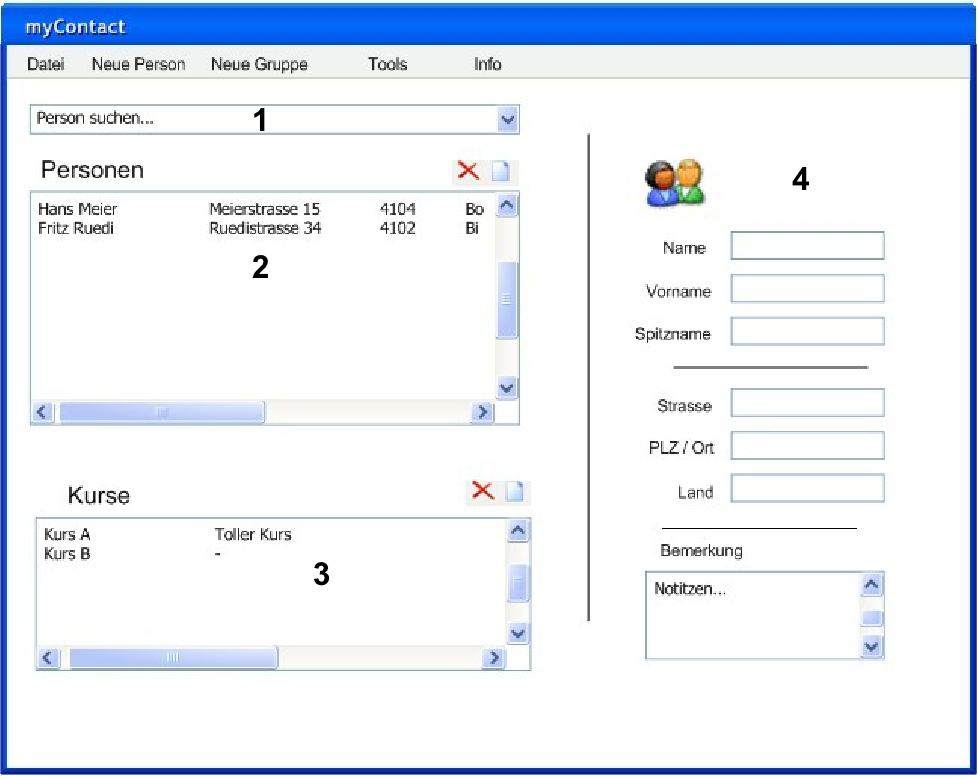
\includegraphics[width=15cm]{images/main.png}
\caption{Startseite der Applikation}
\end{center}
\end{figure}
%
Das Hauptfenster ist in 4 Bereiche gegliedert. Es ist das einzige Frame, alle anderen
Fenster werden Dialoge sein.\\
\\
\textbf{Bereich 1}\\
Hier kann man nach einer Person suchen.
\\[2ex]
\textbf{Bereich 2}\\
Liste von Personen, die auf die Suche zutreffen. Wenn nichts in der Suche angezeigt wird,
werden alle vorhandenen Personen in der Liste angezeigt.
\\[2ex]
\textbf{Bereich 3}\\
Liste von Kursen. Ist eine Person ausgewählt, werden nur noch die Kurse angezeigt, die
die Person besucht hat.
\\[2ex]
\textbf{Bereich 4}\\
Detailinformationen über die Person, die man im Bereich 2 ausgewählt hat.
\\[2ex]
\begin{figure}[ht]
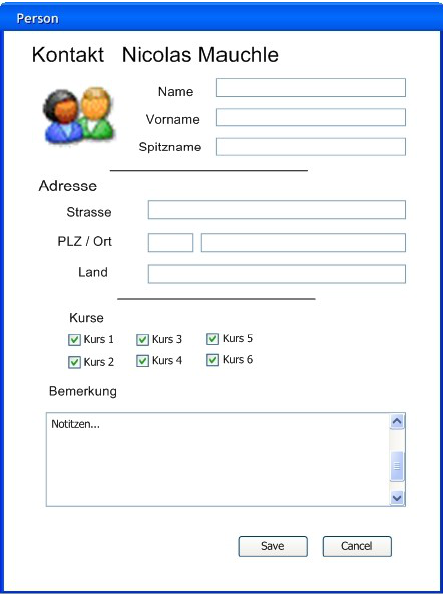
\includegraphics[width=10cm]{images/editPerson.png}
\caption{Fenster: Personen bearbeiten}
\end{figure}
\\[2ex]
\textit{Info zu Kursen:}\\
Hier sind alle Kurse aufgelistet, wenn ein Häkchen bei einem Kurs gemacht wird, ist diese
Person bei diesem Kurs dabei.
\\
\begin{figure}[ht]
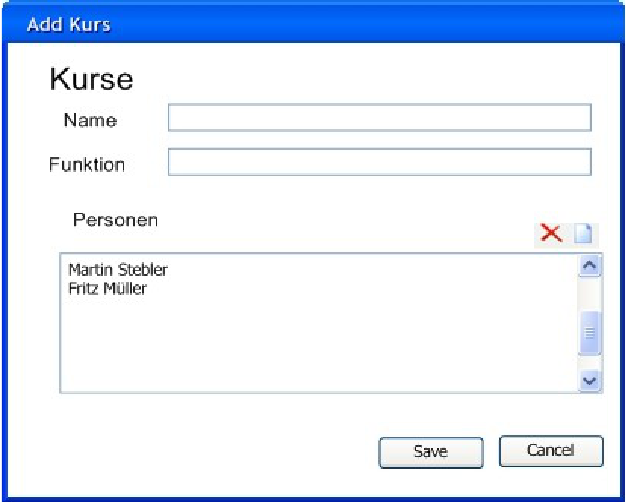
\includegraphics[width=10cm]{images/editCourse.png}
\caption{Fenster: Kurse bearbeiten}
\end{figure}
%
\begin{figure}[ht]
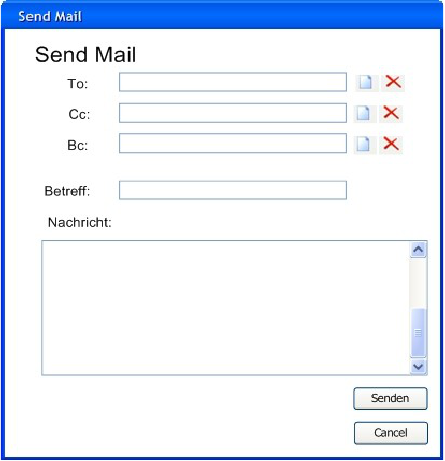
\includegraphics[width=10cm]{images/sendMail.png}
\caption{Fenster: Mail versenden}
\end{figure}
\clearpage

\begin{figure}[ht]
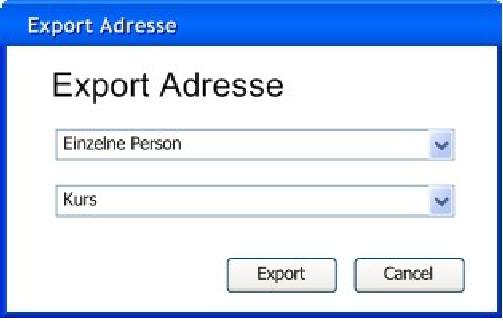
\includegraphics[width=10cm]{images/exportAddress.png}
\caption{Fenster: Adressen exportieren}
\end{figure}
\clearpage

\section{Use-Case}
%
\begin{figure}[ht]
\begin{center}
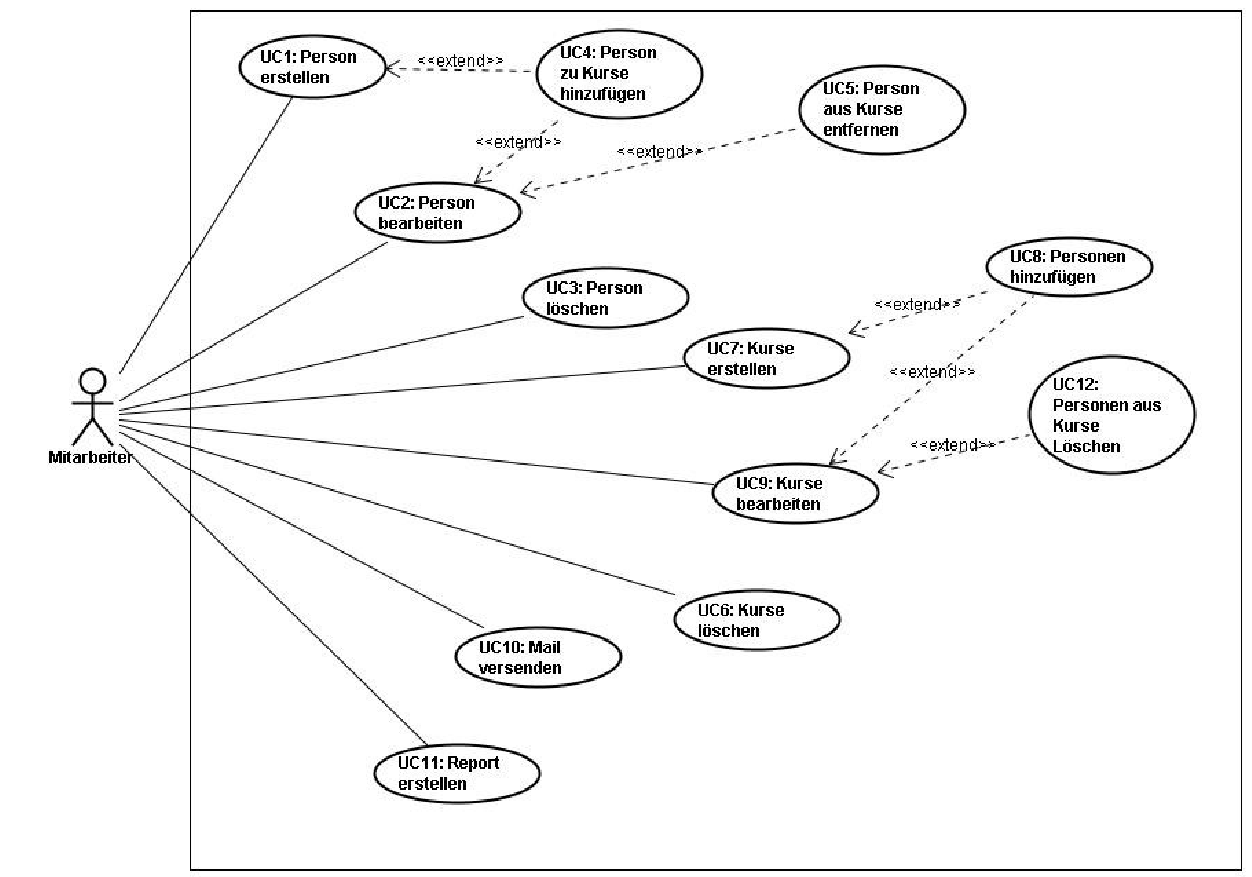
\includegraphics[width=15cm]{images/use-case.png}
\caption{Use-Case Diagramm}
\end{center}
\end{figure}
\clearpage
\textbf{Beschreibung des Geschäftsfalls}
\begin{table}[ht]
\caption{Use Case: 1}
\begin{tabular}[hl]{|p{15cm}|}
  \hline
  \textbf{UC:} 1\\
  \hline
  \textbf{Titel:}  Person erstellen\\
  \hline
  \textbf{Kurzbescgreibung:}  Eine neue Person wird erstellt\\
  \hline
  \textbf{Vorbedingung:} Alle Informationen über die Person müssen vorhanden sein\\
  \hline
  \textbf{Beschreibung des Ablaufs} Schritte:\\
1. Alle benötigten Daten werden eingegeben\\
Speicherung erfolgreich:\\
- Fenster schliesst sich\\
Speicherung nicht erfolgreich weil:\\
- Daten fehlen\\
- Eine Person mit denselben Angaben existiert bereits in der Datenbank\\
  \hline
  \textbf{Auswirkung}: Eine neue Person wird in die Datenbank abgespeichert\\
  \hline
  \textbf{Anmerkung}\\
  \hline
\end{tabular}
\end{table}
%
\begin{table}[h]
\caption{Use Case: 2}
\begin{tabular}[ht]{|p{15cm}|}
  \hline
  \textbf{UC:} 2\\
  \hline
  \textbf{Titel:} Eine existierende Person bearbeiten\\
  \hline
  \textbf{Kurzbescgreibung:}Eine Person die schon existiert wird bearbeitet\\
  \hline
  \textbf{Vorbedingung:} Person muss in der Datenbank sein\\
  \hline
  \textbf{Beschreibung des Ablaufs:} Schritte:\\
1. Person in der Tabelle auswählen\\
2. Gewünschte Daten abändern\\
Speicherung erfolgreich:\\
- Fenster schliesst sich\\
Speicherung nicht erfolgreich weil:\\
- Daten fehlen\\
- Eine Person mit denselben Angaben existiert bereits in der Datenbank\\
  \hline
  \textbf{Auswirkung} Eine existierende Person wird modifiziert\\
  \hline
  \textbf{Anmerkung}\\
  \hline
\end{tabular}
\end{table}
%
\begin{table}[h]
\caption{Use Case: 3}
\begin{tabular}[ht]{|p{15cm}|}
  \hline
  \textbf{UC:} 3\\
  \hline
  \textbf{Titel} Person löschen\\
  \hline
  \textbf{Kurzbescgreibung} Eine existierende Person wird gelöscht.\\
  \hline
  \textbf{Vorbedingung} Person muss in der Datenbank sein\\
  \hline
  \textbf{Beschreibung des Ablaufs}\\
Schritte:\\
1. Person(en) auswählen\\
2. Lösch-Knopf drücken\\
Löschen erfolgreich\\
- Person(en) wird von der Datenbank gelöscht\\
- Person(en) werden aus den Kursen entfernt\\
  \hline
  \textbf{Auswirkung} Eine oder mehrere Personen werden von der Datenbank entfernt\\
  \hline
  \textbf{Anmerkung} Diese Aktion kann nicht rückgängig gemacht werden\\
  \hline
\end{tabular}
\end{table}
%
%
\begin{table}[h]
\caption{Use Case: 4}
\begin{tabular}[ht]{|p{15cm}|}
  \hline
  \textbf{UC:} 4\\
  \hline
  \textbf{Titel:} Personen zu Kurse hinzufügen\\
  \hline
  \textbf{Kurzbescgreibung} Eine Person zu einem oder mehreren Kurse hinzufügen\\
  \hline
  \textbf{Vorbedingung} Kurs muss in der Datenbank existieren \\
  \hline
  \textbf{Beschreibung des Ablaufs}\\
Schritte:\\
1. Person auswählen oder neu erstellen\\
2. Kurs(e) zur Person hinzufügen\\
Person zu Kurs(e) hinzugefügt\\
- Person wird zu Kurs(e) hinzugefügt\\
  \hline
  \textbf{Auswirkung} Kurs(e) werden zu einer Person hinzugefügt\\
  \hline
  \textbf{Anmerkung} Kurse werden erst nach dem drücken des Speicher-Knopf zur Person\\
  \hline
\end{tabular}
\end{table}
%
%
\begin{table}[h]
\caption{Use Case: 5}
\begin{tabular}[ht]{|p{15cm}|}
  \hline
  \textbf{UC:} 5\\
  \hline
  \textbf{Titel:} Person aus Kurs(e) entfernen\\
  \hline
  \textbf{Kurzbescgreibung:} Eine Person wird aus einem oder mehreren Kurse entfernt\\
  \hline
  \textbf{Vorbedingung:}  Person muss in der Datenbank existieren, sowie muss sie
mindestens bei einem Kurs dabei sein.\\
  \hline
  \textbf{Beschreibung des Ablaufs:}\\
Schritte:\\
1. Person auswählen\\
2. Kurse von Personen löschen\\
Person wird vom Kurs entfernt:\\
- Person von Kurs(en) entfernen\\
  \hline
  \textbf{Auswirkung:} Die Person wird von diesen Kursen entfernt.\\
  \hline
  \textbf{Anmerkung:} Diese Aktion kann man nicht rückgängig machen\\
  \hline
\end{tabular}
\end{table}
%
\begin{table}[h]
\caption{Use Case: 6}
\begin{tabular}[ht]{|p{15cm}|}
  \hline
  \textbf{UC:} 6\\
  \hline
  \textbf{Titel:} Kurs(e) löschen\\
  \hline
  \textbf{Kurzbescgreibung:} Einen oder mehrere Kurse löschen\\
  \hline
  \textbf{Vorbedingung:} Kurs muss existieren\\
  \hline
  \textbf{Beschreibung des Ablaufs:}\\
Schritte:\\
1. Kurs im Hauptfenster auswählen\\
2. Auf 'Löschen' drücken\\
Löschen erfolgreich:\\
- Fenster schliesst sich.\\
  \hline
  \textbf{Auswirkung:} Ein neuer Kurs wird erstellt\\
  \hline
  \textbf{Anmerkung:}\\
  \hline
\end{tabular}
\end{table}
%
%
\begin{table}[h]
\caption{Use Case: 7}
\begin{tabular}[ht]{|p{15cm}|}
  \hline
  \textbf{UC:} 7\\
  \hline
  \textbf{Titel:} Kurse erstellen\\
  \hline
  \textbf{Kurzbescgreibung:} Einen neuen Kurs erstellen.\\
  \hline
  \textbf{Vorbedingung:} -\\
  \hline
  \textbf{Beschreibung des Ablaufs:}\\
Schritte:\\
1. Im Menü neuer Kurs auswählen\\
2. Daten eingeben\\
3. [Personen hinzufügen]\\
Speicherung erfolgreich:\\
- Fenster schliesst sich.\\
Speicherung nicht erfolgreich weil:\\
- Daten fehlen\\
  \hline
  \textbf{Auswirkung:}  Ein neuer Kurs wird erstellt\\
  \hline
  \textbf{Anmerkung:}\\
  \hline
\end{tabular}
\end{table}
%
%
\begin{table}[h]
\caption{Use Case: 8}
\begin{tabular}[ht]{|p{15cm}|}
  \hline
  \textbf{UC:} 8\\
  \hline
  \textbf{Titel:} Person zu Kurse hinzufügen\\
  \hline
  \textbf{Kurzbescgreibung:} Eine Person wird zu einem bestehenden Kurs hinzugefügt\\
  \hline
  \textbf{Vorbedingung:} Kurs, sowohl auf Person muss existieren\\
  \hline
  \textbf{Beschreibung des Ablaufs:}\\
Schritte:\\
1. Kurs auswählen\\
2. Person(en) aus der Liste auswählen und zum Kurs hinzufügen\\
3. Speichern\\
Hinzufügen erfolgreich:\\
- Fenster schliesst sich\\
Hinzufügen nicht erfolgreich weil:\\
- Person existiert nicht\\
- Falsche Handhabung\\
  \hline
  \textbf{Auswirkung:} Eine oder mehrere Personen werden zu einem Kurs hinzugefügt\\
  \hline
  \textbf{Anmerkung:}\\
  \hline
\end{tabular}
\end{table}
%
%
\begin{table}[t]
\caption{Use Case: 10}
\begin{tabular}[ht]{|p{15cm}|}
  \hline
  \textbf{UC:} 10\\
  \hline
  \textbf{Titel:} Mail versenden\\
  \hline
  \textbf{Kurzbescgreibung:} Nachrichten an Personen oder an Kursteilnehmer senden.\\
  \hline
  \textbf{Vorbedingung:} Personen existieren in der Datenbank sowie auch Kurse\\
  \hline
  \textbf{Beschreibung des Ablaufs:}\\
Schritte:\\
1. Felder ausfüllen die benötigt werden:\\
- To\\
- CC\\
- Bc\\
- Betreff\\
- Nachricht\\
2. Senden-Knopf drücken\\
Mail wird versendet :\\
- Nachricht kommt, dass das Mail versendet wurde. - Bestätigung\\
- Fenster schliesst sich.\\
Mail wird nicht versendet weil:\\
- To-Feld wurde nicht ausgefüllt.\\
  \hline
  \textbf{Auswirkung:} Ein Mail wird an Personen die man ausgewählt hat versendet\\
  \hline
  \textbf{Anmerkung:}Hier muss man aufpassen, dass man nicht zu viele Mails versendet
(Spam-Gefahr)\\
  \hline
\end{tabular}
\end{table}
%
\\
\textit{UC 9} ist fast gleich wie \textit{UC 2, UC 12} ist fast gleich wie\textit{ UC 5, UC 11} ist fast gleich wie
\textit{UC 10}. Unterschied ist, dass es andere Objekte sind. Vom vorgehen genau gleich.
%
\clearpage
\section{Klassendiagramm}
Es gibt ein Controller, der die Person-Klasse und Course-Klasse verwaltet. Dazu hat die
Person-Klasse die Klasse Contact, die sie verwaltet. Jede Person hat einen Contact.
Der Controller hat mehrere Personen, sowie auch mehrere Kurse(Course).
%
\begin{figure}[ht]
\begin{center}
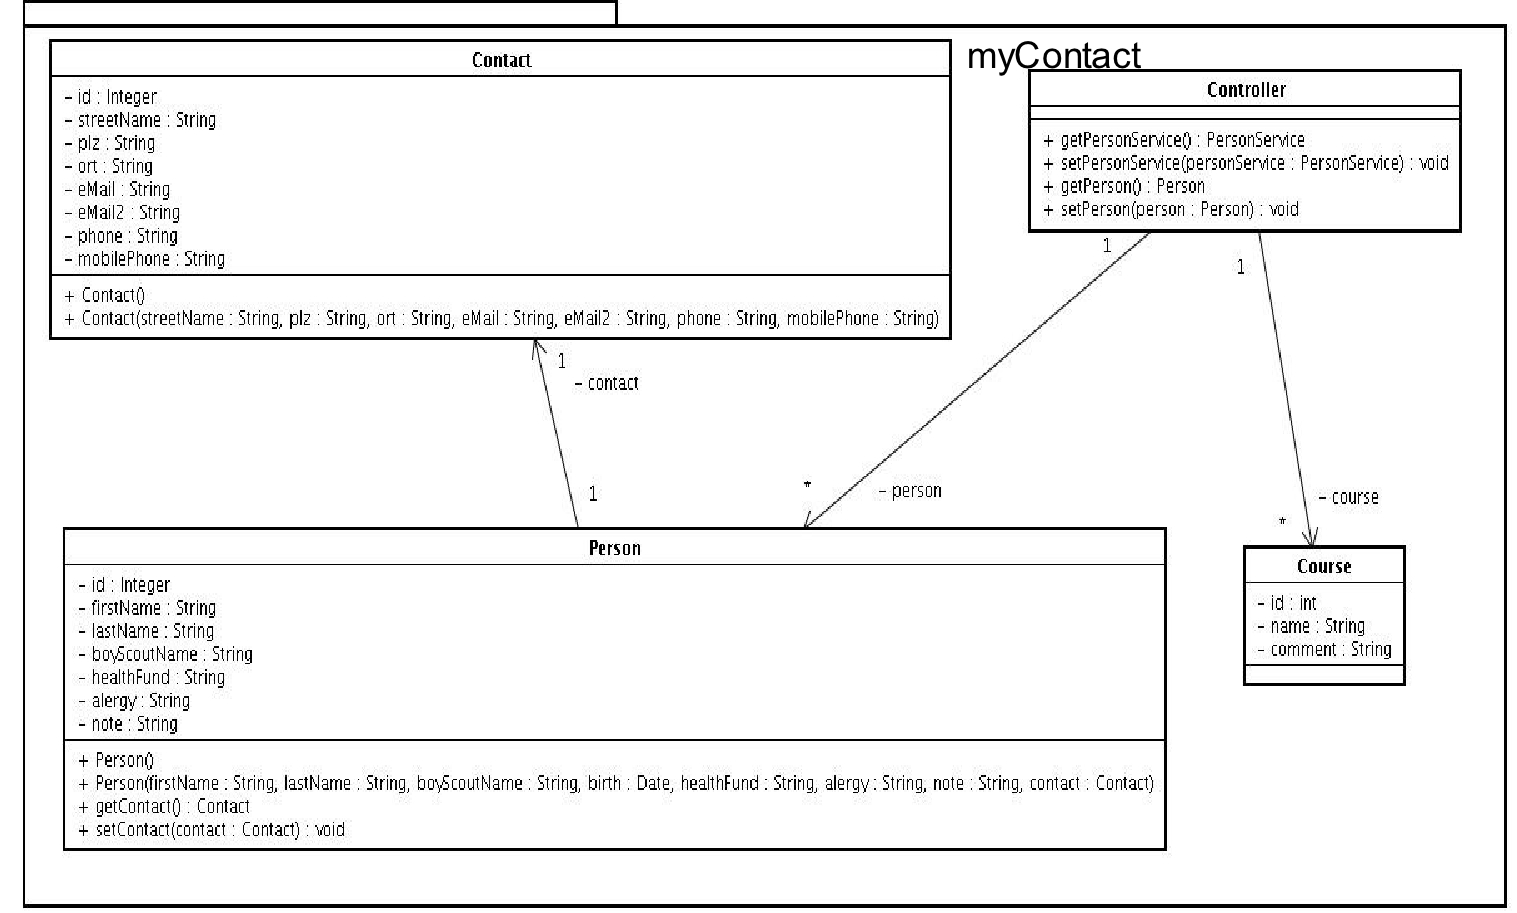
\includegraphics[width=15cm]{images/classDiagramm.png}
\caption{Klassen-Diagramm der Applikation}
\end{center}
\end{figure}
%
\clearpage
\section{Sequenzdiagramm}
\subsection{Applikation starten}
\begin{figure}[ht]
\begin{center}
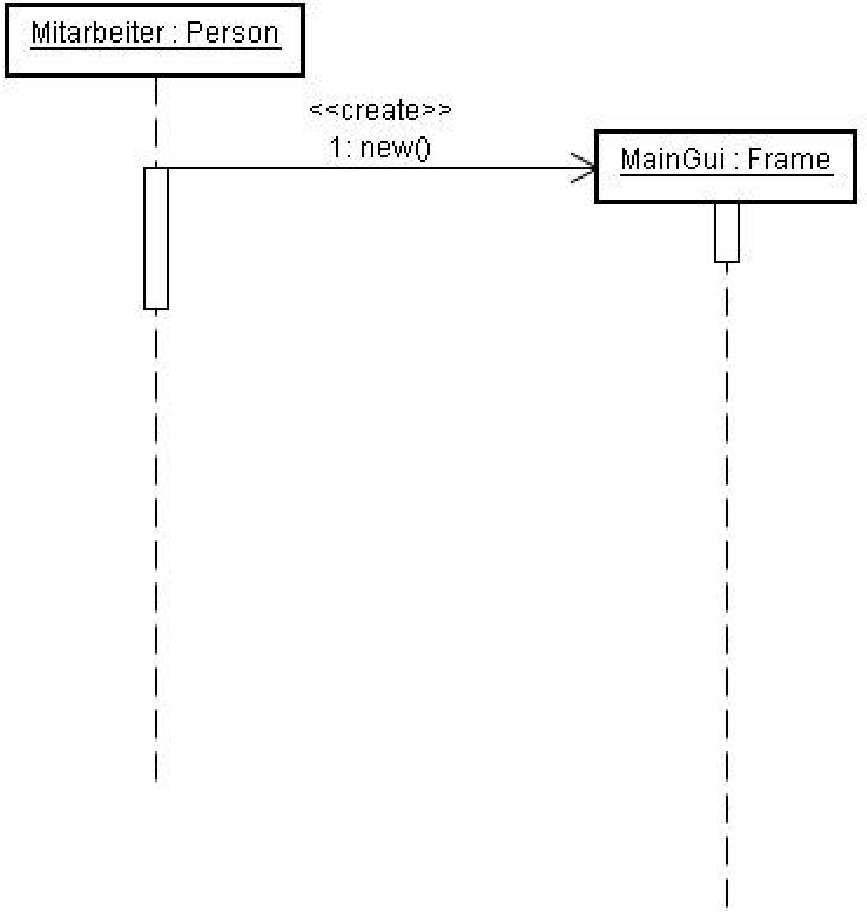
\includegraphics[width=8cm]{images/startApplication.png}
\caption{Sequenzdiagramm: Start der Applikation}
\end{center}
\end{figure}
Die Person startet das Programm. Danach wird das MainGui als Typ Frame ins Leben
gerufen.
%
\clearpage
\subsection{Save person}
\begin{figure}[ht]
\begin{center}
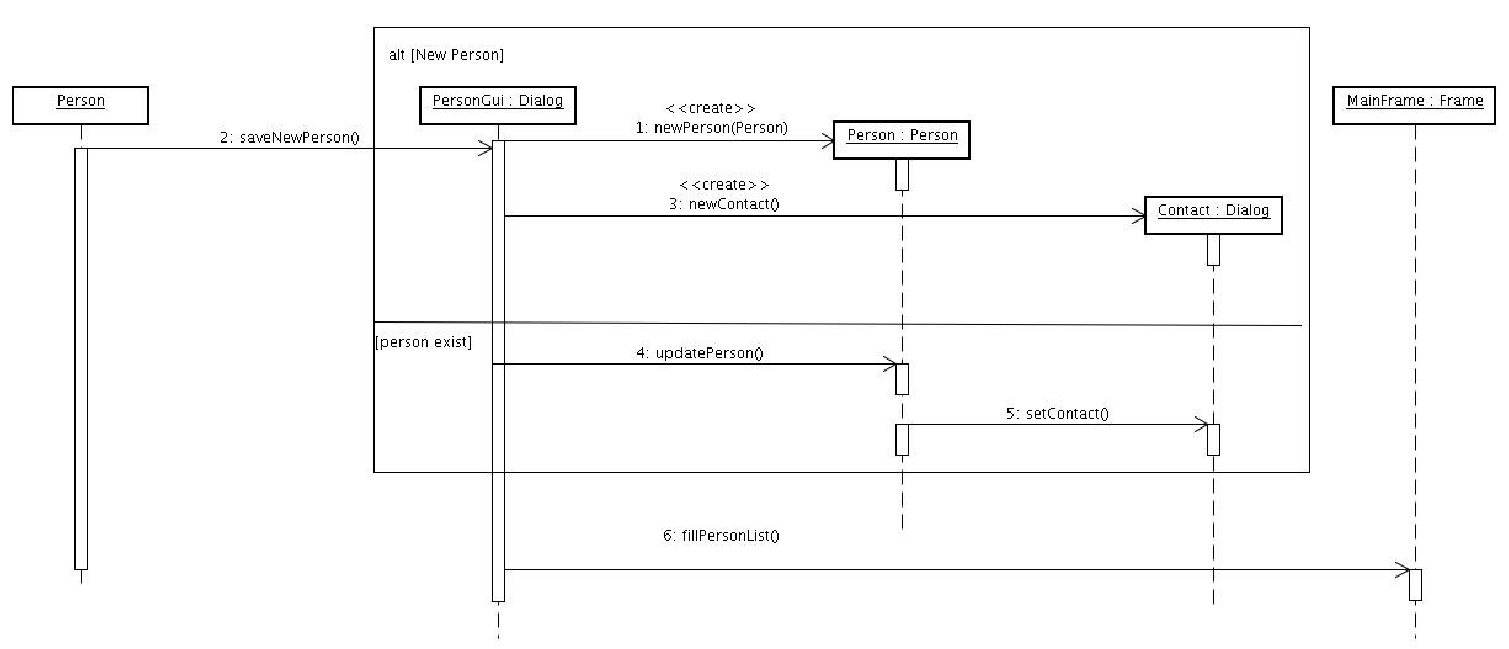
\includegraphics[width=15cm]{images/savePerson.png}
\caption{Sequenzdiagramm: Save Person}
\end{center}
\end{figure}
%
Eine Person speichert eine Person, und führt die Funktion \textit{savePerson} aus. Danach gibt
es zwei Möglichkeiten.
%
\begin{enumerate}
\item Möglichkeit:\\
Eine neue Person wird abgespeichert. Für das wird eine neue Person erstellt in der Klasse
Person. Jede Person hat eine Adresse. Deshalb wird von dem PersonGui eine neue
Adresse erstellt. Ist alles erfolgreich erstellt worden, wird die Personenliste im MainGui
aktualisiert.
%
\item Möglichkeit:\\
Die Person existiert schon, sowie auch die Adresse. Deshalb wird keine neue Person
erstellt, sondern die existierende Person aktualisiert, sowie auch ihre Adresse. Auch hier
wird am Schluss die Liste aktualisiert.
\end{enumerate}
%
\clearpage
%
\subsection{Save Course}
\begin{figure}[ht]
\begin{center}
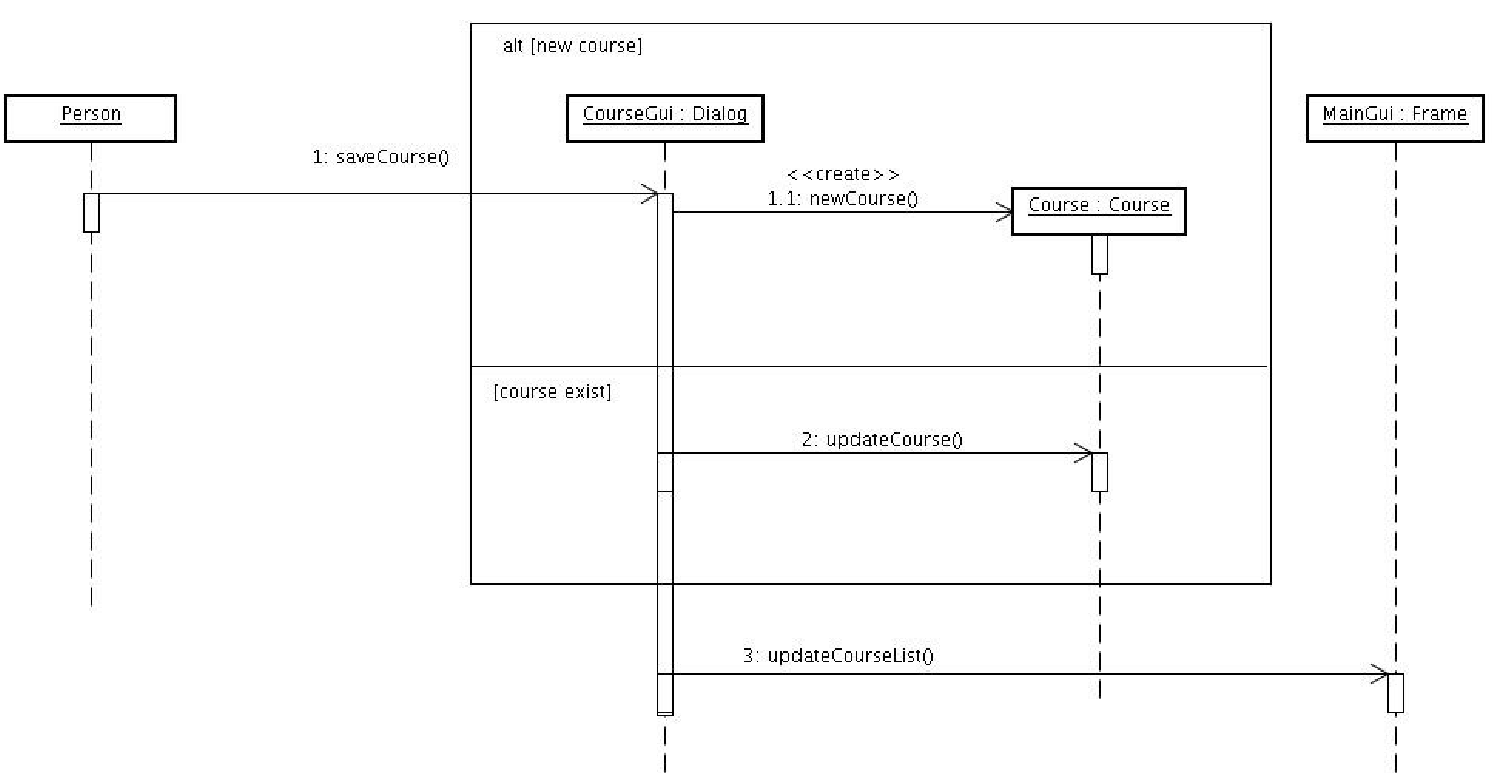
\includegraphics[width=15cm]{images/saveCourse.png}
\caption{Sequenzdiagramm:  Kurse abspeichern}
\end{center}
\end{figure}
Eine Person speichert ein Kurs und führt die Funktion \textit{saveCourse} aus. Danach gibt es
zwei Möglichkeiten.
\begin{enumerate}
\item Möglichkeit:\\
Ein neuer Kurs wird erstellt und nachher die Liste der Kurse im MainGui aktualisiert.
%
\item Möglichkeit:\\
Der Kurs existiert schon und wird aktualisiert. Auch hier wird nachträglich die Kursliste im
MainGui aktualisiert.
\end{enumerate}
\clearpage
\section{Aktivitätsdiagramm}
\subsection{Neue Person hinzufügen}
\begin{figure}[ht]
\begin{center}
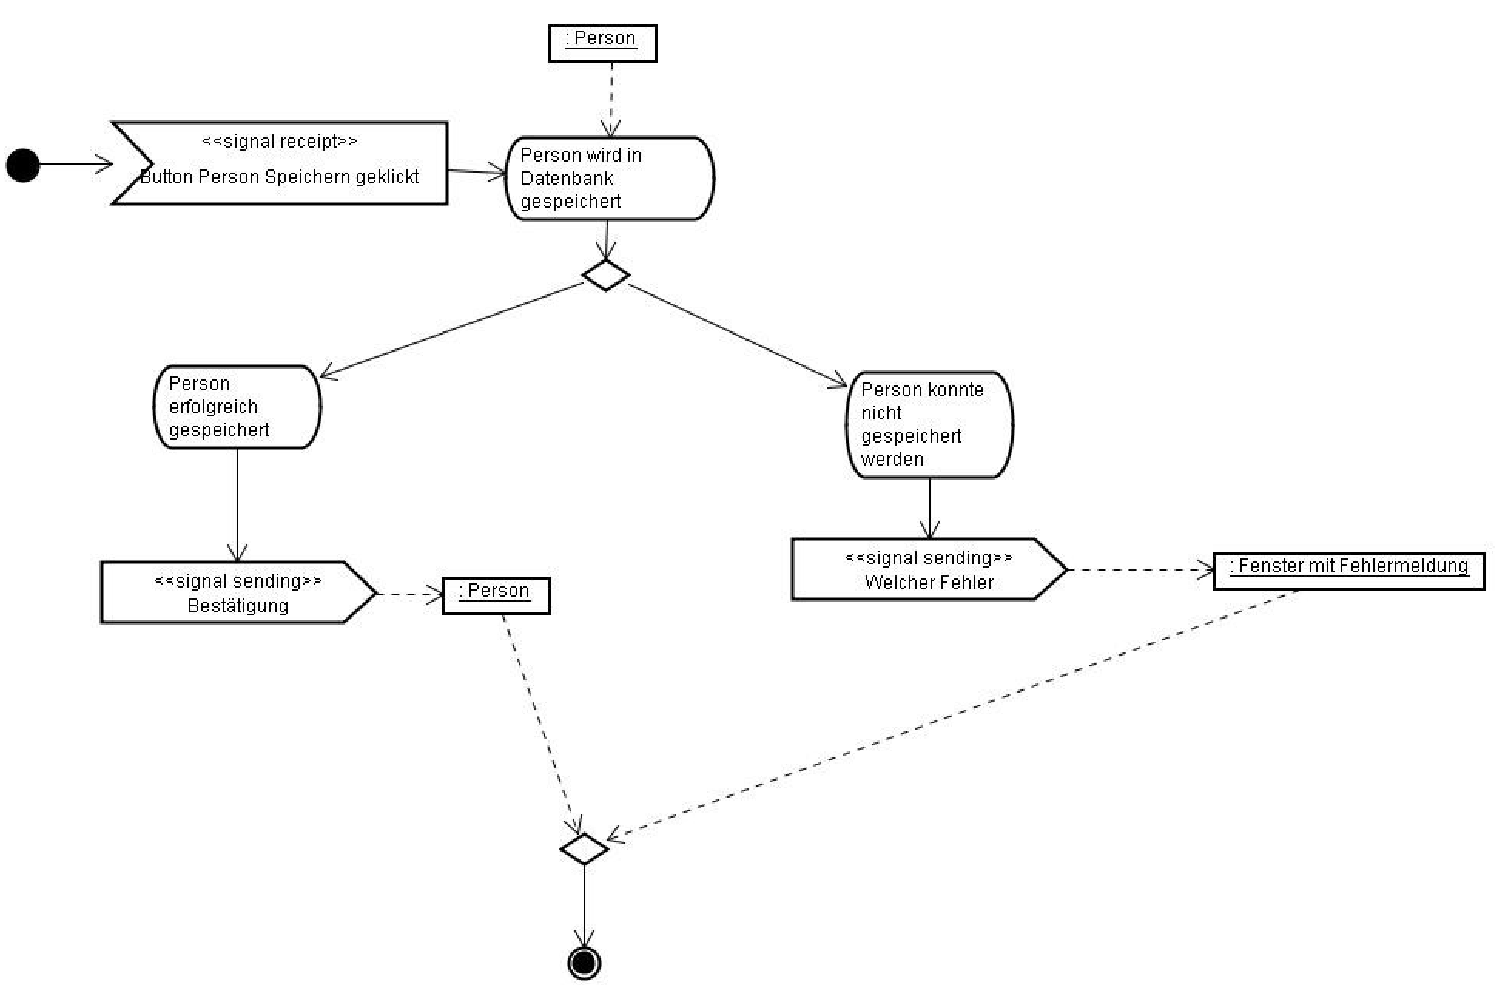
\includegraphics[width=15cm]{images/savePersonAkt.png}
\caption{Aktivitätsdiagramm:  Neue Person speichern}
\end{center}
\end{figure}
Eine neue Person wird erstellt, indem man im GUI auf den 'Speichern' Knopf drückt. Die
Person wird in die Datenbank gespeichert. Entweder funktioniert alles. Das Programm gibt
dann die erstellte Person zurück. Funktioniert es nicht, kommt ein Fenster mit einer
Fehlermeldung.
%
\newpage
\subsection{Person bearbeiten}
\begin{figure}[ht]
\begin{center}
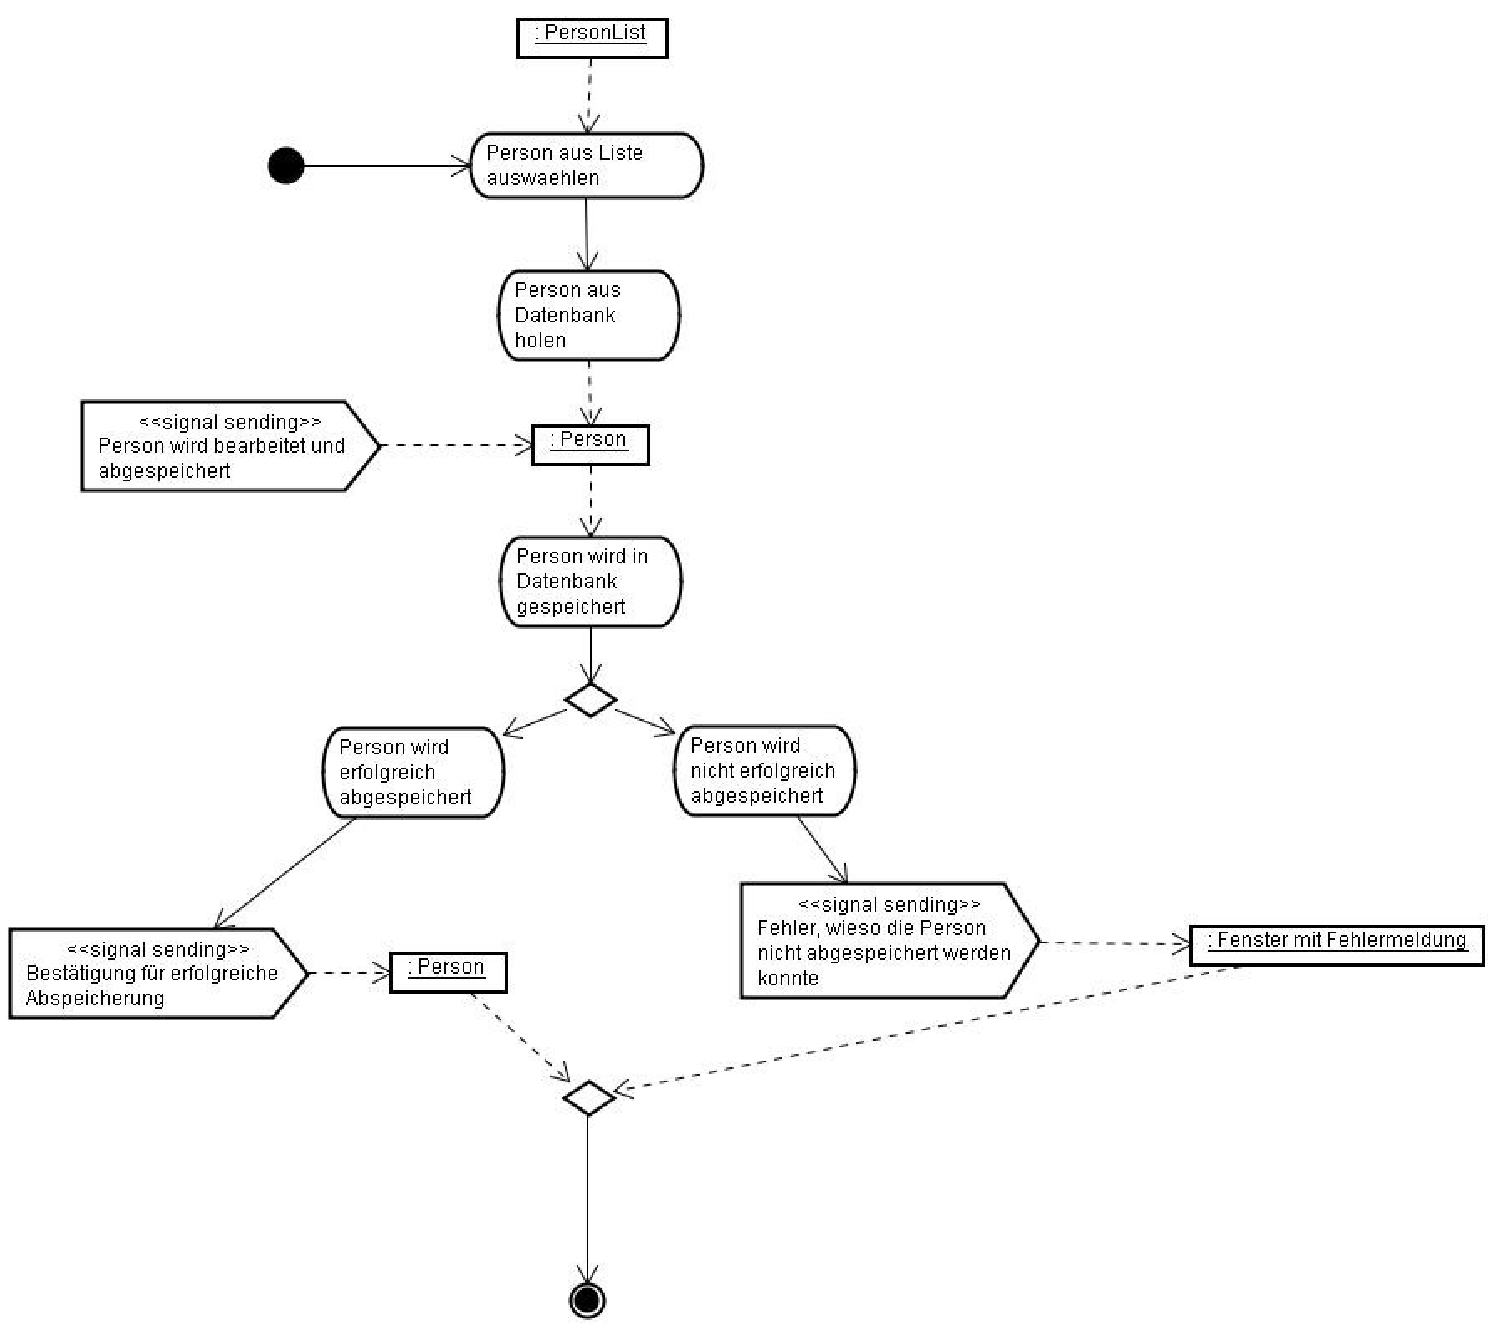
\includegraphics[width=13cm]{images/personakt.png}
\caption{Aktivitätsdiagramm:  Bestehende Person bearbeiten}
\end{center}
\end{figure}
Eine Person wird aus der Personenliste ausgewählt. Somit müssen jetzt alle Attribute aus
der Datenbank gelesen werden. Danach kann man die erhaltene Person bearbeiten. Der
Ablauf ist jetzt gleich wie bei 'Person speichern'.
\clearpage
